% 
% Annual Cognitive Science Conference
% Sample LaTeX Paper -- Proceedings Format
% 

% Original : Ashwin Ram (ashwin@cc.gatech.edu)       04/01/1994
% Modified : Johanna Moore (jmoore@cs.pitt.edu)      03/17/1995
% Modified : David Noelle (noelle@ucsd.edu)          03/15/1996
% Modified : Pat Langley (langley@cs.stanford.edu)   01/26/1997
% Latex2e corrections by Ramin Charles Nakisa        01/28/1997 
% Modified : Tina Eliassi-Rad (eliassi@cs.wisc.edu)  01/31/1998
% Modified : Trisha Yannuzzi (trisha@ircs.upenn.edu) 12/28/1999 (in process)
% Modified : Mary Ellen Foster (M.E.Foster@ed.ac.uk) 12/11/2000
% Modified : Ken Forbus                              01/23/2004
% Modified : Eli M. Silk (esilk@pitt.edu)            05/24/2005
% Modified : Niels Taatgen (taatgen@cmu.edu)         10/24/2006
% Modified : David Noelle (dnoelle@ucmerced.edu)     11/19/2014
% Modified : Roger Levy (rplevy@mit.edu)     12/31/2018



%% Change "letterpaper" in the following line to "a4paper" if you must.

\documentclass[man,floatsintext]{apa6}


%\cogscifinalcopy % Uncomment this line for the final submission 


\usepackage{pslatex}
\usepackage{apacite}
\usepackage{graphicx}
\usepackage{colortbl}
\usepackage{tikz}
\graphicspath{ {./plots/} }
\usepackage{float} % Roger Levy added this and changed figure/table
                   % placement to [H] for conformity to Word template,
                   % though floating tables and figures to top is
                   % still generally recommended!

%\usepackage[none]{hyphenat} % Sometimes it can be useful to turn off
%hyphenation for purposes such as spell checking of the resulting
%PDF.  Uncomment this block to turn off hyphenation.


%\setlength\titlebox{4.5cm}
% You can expand the titlebox if you need extra space
% to show all the authors. Please do not make the titlebox
% smaller than 4.5cm (the original size).
%%If you do, we reserve the right to require you to change it back in
%%the camera-ready version, which could interfere with the timely
%%appearance of your paper in the Proceedings.

\usepackage{booktabs}
\usepackage{color}
\definecolor{LightGray}{gray}{0.92}
\definecolor{Purple}{RGB}{147, 0, 163}
\newcommand{\purple}[1]{\textcolor{Purple}{#1}}
\newcommand{\jd}[1]{\textcolor{Purple}{\bf [jd: #1]}}
\definecolor{Red}{RGB}{163, 0, 0}
\newcommand{\red}[1]{\textcolor{Red}{#1}}
\newcommand{\seb}[1]{\textcolor{Red}{\bf [Seb: #1]}}
\definecolor{Green}{RGB}{0, 176, 76}
\newcommand{\ml}[1]{\textcolor{Green}{\bf [ml: #1]}}

%\renewcommand{\cite}[1]{(\textbf{#1})}

\title{Explaining away in semantic-pragmatic adaptation}
\shorttitle{Explaining away in semantic-pragmatic adaptation}
  
\author{Sebastian Schuster, Matthew Iver Loder, and Judith Degen}
\affiliation{Department of Linguistics, Stanford University}


\abstract{Previous work has shown that listeners deal with variability in language use through adaptation; they update expectations about a specific speaker's productions based on the interactions with that speaker. We explore whether contextual information such as a speaker's mood can influence the extent to which listeners adapt to variable use of uncertainty expressions like \textit{might} and \textit{probably}. We find that information about the speaker's mood influences participants' expectations about a generic speaker's use of uncertainty expressions (Exp.~1). We further find that information about the speaker's mood influences adaptation behavior: listeners adapt less to a speaker if they are provided with a reason for the observed language use (Exp.~2), though not more when the behavior is highly unexpected (Exp.~3).  These results suggest that listeners explain away otherwise unexpected behavior when presented with a reason,  and that the extent of adaptation depends on prior expectations about language use.}

\keywords{adaptation; semantics; pragmatics; uncertainty expressions, explaining away}

\begin{document}

\maketitle



\section{Introduction}

Variability across speakers can be observed at all levels of linguistic representation and no two speakers use language exactly the same way. For example, at the lexical level, one speaker may use the  quantifier \textit{some} to describe a proportion of about 50\% whereas another speaker may use the quantifier \textit{many} in that situation \cite{Yildirim2016}. Listeners deal with this variability by adapting to individual speakers and forming speaker-specific expectations about language use \cite[inter alia]{Norris2003,Kraljic2005,Bradlow2008,Kurumada2012,Kamide2012,Kleinschmidt2015,Fine2016,Roettger2019}. For example, for utterances with quantifiers,  \citeA{Yildirim2016} found that this variability was reflected in participants' initial beliefs about the use of quantifiers: participants were uncertain whether a generic speaker would use the utterance \textit{Some of the candies are green} or the utterance \textit{Many of the candies are green} to describe a bowl in which there were approximately equal numbers of green and blue candies. However, if participants briefly observed a speaker describing this scene either consistently using \textit{some} or consistently using \textit{many}, they updated their expectations about how that speaker would use quantifiers to describe different proportions to closely mirror the observed speaker's usage. Similarly, \citeA{Schuster2020} found that listeners update their expectations about a speaker's mapping between uncertainty expressions like \textit{might} or \textit{probably} and event probabilities after brief exposure to that speaker; when exposed to a speaker who consistently used \textit{might} to describe an event probability of 60\%, participants expected the speaker to use \textit{might} for higher event probabilities than when when exposed to a speaker who consistently used \textit{probably} to describe the same event probability.

Most investigations into how listeners adapt so far have been based on the assumption that a lot of the variability is \textit{intrinsic} to the speaker and does not vary across contexts. This assumption is reasonable for many kinds of variability. For example, a lot of acoustic properties of productions are determined by a combination of the speaker's gender and the geographical region that they grew up in \cite{Kleinschmidt2019}, which are both properties of the speaker that generally do not change between contexts. If one interacts with a woman with a Brooklyn accent, it is highly unlikely that she will sound like an average male speaker with a Southern accent the next time one talks to her. Or, returning to the lexical level, if one interacts with a speaker whose semantic representation of the quantifier \textit{a couple of} is equivalent to the representation of \textit{exactly two}, it is unlikely that they would suddenly use \textit{a couple of} to refer to small quantities greater than two.

At the same time, however, variability in language use can often be attributed to contextual factors other than the speaker, and listeners consider these factors in interpretations. 
For example, the interpretation of quantifiers and uncertainty expressions depends on the distribution over quantities and base probability rates: \textit{a few mountains} is generally interpreted to refer to a lower quantity than \textit{a few crumbs} \cite{Clark1991,Scholler2017} and \textit{probably} describing the likelihood of snow in the North Carolina mountains in December is generally interpreted to describe higher event probabilities than when \textit{probably} is used to indicate the likelihood of snow in October \cite{Wallsten1986b}. Similarly, perceived social goals such as being polite affect interpretations. \cite{Pighin2011} found that uncertainty expressions used to convey the likelihood of an undesirable medical outcome were interpreted to refer to higher event probabilities than when the same expression was used to convey the likelihood of a desirable outcome, presumably because listeners attributed the use of the uncertainty expression to sugarcoating an potentially upsetting truth.

Considering that variability in use can sometimes but not always be attributed to a specific speaker, it would be beneficial for listeners to selectively adapt to speakers only when variability cannot be attributed to other contextual factors. To what extent this is happening and to what extent contextual factors modulate listener's adaptive behavior is the focus of the work presented here. 

To illustrate how contextual factors may modulate adaptive behavior, consider a speaker $S$ who is in a very good mood and wants to be encouraging. If $S$ tells a listener $L$ ``you'll \textit{probably} win the sweepstake'' when there is only a 60\% chance of winning, $L$ may consider $S$'s use of \textit{probably} instead of a weaker alternative such as \textit{might} to be the result of $S$'s mood. Consequently, $L$ would not necessarily expect $S$ to use \textit{probably} to describe the same event probability when $S$ is in a worse or more discouraging mood.

%To illustrate this, consider a listener who encounters a used car salesman describing obviously mediocre cars with highly positive adjectives such as \textit{amazing}. Being aware of the speaker's incentive to use extremely positive language, the listener will likely not update their beliefs about the speaker's use of evaluative adjectives, and for example, if the same speaker later recommends an ``amazing restaurant'', the listener will likely not conclude that the restaurant is actually mediocre.

Recent computational models suggest that such modulation is possible. \citeA{Schuster2020}  proposed a computational model of adaptation to variable use of uncertainty expressions based on Bayesian belief updating. According to this model, when interacting with a speaker and observing their language use, listeners integrate their prior beliefs about the speaker's semantic representations and lexical preferences with the observed utterances to arrive at updated speaker-specific production expectations. Similar Bayesian belief-updating models have been proposed for adaptation in other linguistic domains, including in phonetic adaptation \cite{Kleinschmidt2015}, syntactic adaptation \cite{Kleinschmidt2012}, and prosodic adaptation \cite{Roettger2019}. All of these models predict that the extent to which listeners adapt depends on how they initially expect a speaker to use language. Consequently, contextual factors that affect listeners' expectations about language use should also affect how much listeners adapt to specific speakers. If, given contextual information, a speaker's behavior matches prior expectations, there is no need to adapt.



In addition to the model-predicted influence of contextual factors on adaptation, there is  empirical evidence from phonetic adaptation: \citeA{Kraljic2008} used a lexical retuning paradigm to investigate adaptation to a speaker who produced a sound that was ambiguous between /s/ and /sh/. They found that without additional information listeners adapted, such that their perceptual boundary between /s/ and /sh/ shifted. However, when participants were shown a picture of the speaker with a pencil in their mouth, they explained away the observed signal as a pencil-distorted /sh/-sounding /s/ rather than as an intentionally produced /sh/-sounding /s/. Consequently, they did not adapt, i.e., their perceptual boundary between /s/ and /sh/ did not shift.

In this work, we investigate for the first time whether listeners explain away otherwise unexpected behavior at the lexical level if they are presented with contextual information that provides a reason for a speaker's productions. Concretely, we investigate whether one contextual factor  -- the speaker's mood -- provides such a reason for otherwise less expected uses of the uncertainty expressions \textit{might} and \textit{probably}  (\textsc{explaining away hypothesis}). However, considering that previous experimental studies on semantic-pragmatic adaptation \cite{Yildirim2016,Schuster2020} kept all aspects of the context constant between the exposure and test phase, it could also be that listeners simply learn associations between the use of uncertainty expressions and speakers, independent of other contextual information (\textsc{associative hypothesis}).

We first discuss how additional contextual factors can be modeled within the computational framework proposed by \citeA{Schuster2020} and how this model may lead to "explaining away" \cite{Pearl1988} of otherwise unexpected variability (Section~2).  We then investigate this issue empirically as follows. We first establish that language users have different expectations about a generic speaker's use of uncertainty expressions depending on their beliefs about the speaker's mood (Exp.~1, Section~3). We then investigate how much participants adapt when they are provided with information about the speaker's mood that makes their use of uncertainty expressions more expected, and compare participants' adaptation behavior to a neutral adaptation setting in which participants do not receive any information about the speaker's mood (Exp.~2, Section~4). Finally, we investigate the relationship between adaptation and highly unexpected behavior by exposing participants to a speaker whose use of uncertainty expressions is incongruent with their mood (Exp.~3, Section~4). We find that listeners adapt less when they are presented with a reason for the speaker's behavior. However, surprisingly, we also find that listeners do not adapt more when the behavior is highly unexpected given contextual information, potentially suggesting that listeners draw additional inferences when encountering highly unexpected behavior or that there are limits on adaptation.

\section{Modeling explaining away}
\label{sec:model}

In this section, we first briefly review the Bayesian belief updating model of semantic adaptation that will form the basis of the explaining away model. We then review the concept of explaining away in probabilistic graphical models, and finally we show how additional contextual factors can be integrated into the belief updating model and how the resulting model gives rise to explaining away.

\paragraph{Bayesian belief updating model} \citeA{Schuster2020} present a Bayesian cognitive model at the computational level \cite{Marr1982,Anderson1990} of how listeners adapt to variable use of uncertainty expressions. The core idea of this model is that listeners have beliefs about how a generic speaker would use uncertainty expressions to describe probabilities of a future event and that in interaction, when listeners observe a specific speaker's behavior, they refine their beliefs starting off from the beliefs about the generic speaker to better match that speaker's language use. More formally, this model assumes that listeners have beliefs about speaker-specific parameters $\Theta_S$ in the form of a distribution $P(\Theta_S)$. Given observations $O$ about the use of uncertainty expressions, listeners update their beliefs about speaker-specific parameters through Bayesian belief updating:

$$ P(\Theta_S \mid O) \propto P(\Theta_S) P(O \mid \Theta_S) $$

For predicting listeners' expectations about a speaker's language use, \citeA{Schuster2020} employ a probabilistic pragmatic model within the Rational Speech Act framework \cite{Goodman2016}, which is parameterized by the set of speaker-specific parameters $\Theta_S$. $\Theta_S$ is comprised of parameters guiding the semantic representation of uncertainty expressions as well as the speaker preferences for different uncertainty expressions but for the purpose of this work, we limit the discussion to an abstract set of speaker-specific parameters $\Theta_S$ (see the original paper for how individual parameters influence listeners' expectations and interpretations).

As mentioned above, this model was used by  \citeA{Schuster2020} to predict participants' expectations of a speaker and their interpretations after exposure to either a ``\textit{cautious}'' or a ``\textit{confident}'' speaker, whose use of uncertainty expressions differed.  When talking about the probability of getting a blue gumball from a machine filled with orange and blue gumballs,  the ``\textit{cautious}'' speaker always used  ``You \textit{might} get a blue one'' to describe a probability of 60\% and the ``\textit{confident}'' speaker always used ``You'll \textit{probably} get a blue one'' to describe a 60\% probability. This exposure shifted listeners' expectations and this shift is predicted by the model as schematically illustrated in the upper part of Figure~\ref{fig:model-viz}: Listeners start out with their beliefs about a generic speaker (center panel) and depending on the exposure speaker, their expectations about the use of \textit{might} and \textit{probably} either shift to cover higher probabilities (``\textit{cautious}'' speaker, left panel) or lower probabilities (``\textit{confident}'' speaker, right panel). Here and throughout this paper, we assume that an average speaker's use of uncertainty expressions is captured by the parameterization $\Theta_{avg}$, and that the use by ``\textit{cautious}'' or ``\textit{confident}'' speakes are captured by the parameterizations $\Theta_{cau}$ and $\Theta_{con}$. Thus, listeners' beliefs $P(\Theta_S)$ should assign a high probability to $P(\Theta_S = \Theta_{avg})$ prior to exposure and a high probability to $P(\Theta_S = \Theta_{cau})$ or $P(\Theta_S = \Theta_{con})$ after exposure, which is predicted by the belief updating model.


\begin{figure}[th!]
    \centering
    \begin{tikzpicture}

\draw (9.5, 2) node {$\Theta_{cau}$};

\draw (14.75, 2) node {$\Theta_{avg}$};

\draw (20,  2) node {$\Theta_{con}$};

\draw(8,2) node {};

\draw[black,->] (9.5, 1.65) -- (9.5, 1);

\draw[black,->] (14.75, 1.65) -- (14.75, 1);


\draw[black,->] (20, 1.65) -- (20, 1);


\end{tikzpicture}

    \includegraphics[width=\columnwidth]{model-visualization-predictions.pdf}
     \includegraphics[width=\columnwidth]{distribution-combinations.png}
    \caption{\textbf{Top}: Schematic visualization of different parameterizations ($\Theta_{cau}$, $\Theta_{avg}$, $\Theta_{con}$) of the production expectation model. Here we assume that the four possible utterances are ``You won't get a blue one'' (bare not), ``You might get a blue one'' (might), ``You'll probably get a blue one'' (probably), and ``You'll get a blue one'' (bare). The center panel shows the expectations of an average speaker (parameterized by $\Theta_{avg}$) that a listener may assume of a generic speaker that they haven't interacted with. The left and right panels show expectations after exposure to either a ``cautious`` or a ``confident'' speaker, parameterized by $\Theta_{cau}$ and $\Theta_{conn}$, respectively. The vertical dashed line indicates an event probability of 60\%. \\
    \textbf{Bottom}: Schematic distributions over speaker-specific parameters $P(\Theta_S)$ and contextual parameters $P(\Phi_{CTX})$ that lead to expectations in the corresponding upper panels. }
    \label{fig:model-viz}
\end{figure}


\paragraph{Explaining away} The second ingredient to modeling the modulation of additional contextual factors on the adaptation process is the notion of ``explaining away.'' Explaining away is a concept from probabilistic graphical models \cite<PGMs;>{Pearl1988}, a class of models that was originally developed for uncertain reasoning in artificial intelligence systems. PGMs can be used to model causal structures between variables of interest. Figure~\ref{fig:pgm-ex} shows an example of a PGM with three variables representing whether the ground is shaking (\textsc{shake}), whether there is an earthquake (\textsc{quake}), or whether there is a giant roaming around (\textsc{giant}). This PGM further encodes the causal relations between the three variables: if there is an earthquake or a giant roaming around (or both), then the ground is shaking. While earthquakes are very unlikely to occur at any given point in time, it seems reasonable to assume that the sighting of a giant is still much much more unlikely, so the prior probabilities for \textsc{giant} and \textsc{quake} intuitively follow the ordering $P(GIANT) <<< P(QUAKE) <<< 1$. According to this model, if one observes the ground shaking (and if one assumes that \textsc{quake} and \textsc{giant} are the only possible causes for that), then either   \textsc{quake} or \textsc{giant} has to be true, and their respective probabilities will be proportional to their prior probabilities, meaning that in the absence of further information, the likelihood $P(QUAKE)$ will be  close to 1 considering that the prior probability of \textsc{quake} is much greater than the one of \textsc{giant}. This captures the intuition that one is much more likely to attribute a shaking ground to an earthquake than a giant roaming around. However, if one again observes the ground to be shaking but also sees a giant roaming around (and thus the likelihood $P(GIANT)$ is 1), computing $P(QUAKE \mid SHAKE, GIANT)$ according to the structure of this PGM results in a very low likelihood for an earthquake, capturing the intuition that 
if there is already a cause for the ground shaking (the observed giant), then one is unlikely to attribute this observation to a second cause.

\begin{figure}[t]
    \centering
    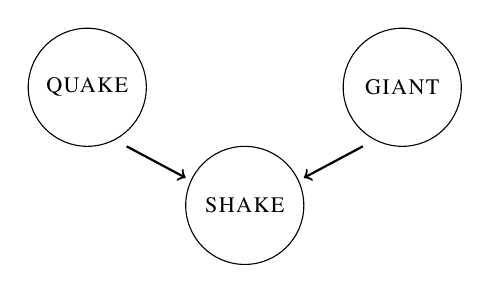
\begin{tikzpicture}
    \draw[black] (-1, 1.5) circle (0.75);
    \draw[black] (-1, 1.5) node {\textsc{quake}};
    
    \draw[black] (3, 1.5) circle (0.75);
    \draw[black] (3, 1.5) node {\textsc{giant}};

    \draw[black] (1, 0) circle (0.75);
    \draw[black] (1, 0) node {\textsc{shake}};

   \draw[black,->,thick] (-0.5, 0.75) -- (0.25, 0.35);
   \draw[black,->,thick] (2.5, 0.75) -- (1.75, 0.35);


    \end{tikzpicture}
    \caption{Example probabilistic graphical model indicating the causal structures between three variables.}
    \label{fig:pgm-ex}
\end{figure}

Apart from modeling causal reasoning in probabilistic artificial agents, explaining away has also been argued to apply to several phenomena in cognition, including visual object recognition \cite{Murray2002} and priming in word recognition experiments \cite{Huber2008}. Somewhat surprisingly though considering that PGMs were designed for causal reasoning, explaining away does not seem to properly capture human causal reasoning behavior in many instances \cite[inter alia]{Morris1995,Tenenbaum2002,Rehder2017}. It thus remains an open question how commonly explaining away predicts cognitive behavior to what extent explaining away happens in semantic-pragmatic adaptation.

\paragraph{Explaining away in semantic-pragmatic adaptation.} As we mentioned above, according to the  belief-updating model, listeners update their beliefs about speaker-specific parameters $P(\Theta_S)$ that guide their production expectations. Here, we extend this model and assume that that listeners expectations are not only guided by their beliefs about speaker-specific parameters, $P(\Theta_S)$, but also by their beliefs about other contextual factors, $P(\Phi_{CTX})$. The resulting combination of factors, $P(\Psi_{S+CTX})$, is shown in the graphical model in Figure~\ref{fig:explaining-away-model}.\footnote{We leave it open how exactly beliefs about speaker-specific and other contextual parameters are combined. One  possibility is that they are linearly combined like parameters in a linear model but theoretically, they could be combined through any mathematical function.}

\begin{figure}[t]
    \centering
    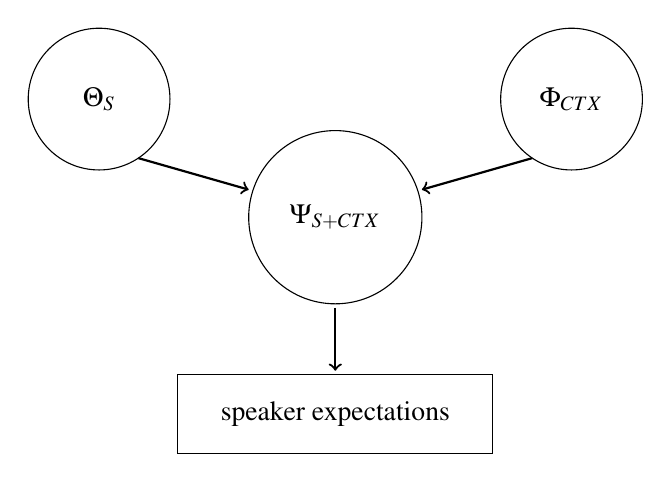
\begin{tikzpicture}
    \draw[black] (-2, 1.5) circle (0.9);
    \draw[black] (-2, 1.5) node {$\Theta_S$};
    
    \draw[black] (4, 1.5) circle (0.9);
    \draw[black] (4, 1.5) node {$\Phi_{CTX}$};

    \draw[black] (1, 0) circle (1.1);
    \draw[black] (1, 0) node {$\Psi_{S+CTX}$};

   \draw[black,->,thick] (-1.5, 0.75) -- (-.1, 0.35);
   \draw[black,->,thick] (3.5, 0.75) -- (2.1, 0.35);
 
       \draw[black,->,thick] (1, -1.15) -- (1, -1.95);


    \draw[black] (-1, -3) rectangle (3,-2);
    \draw[black] (1, -2.5) node {speaker expectations};


    \end{tikzpicture}
    \caption{Probabilistic graphical model showing how speaker-specific ($\Theta_S$) and other contextual ($\Phi_{CTX}$) parameters are combined to form the parameters $\Psi_{S+CTX}$ guiding expectations about a speaker's use of uncertainty expressions in a specific context.}
    \label{fig:explaining-away-model}
\end{figure}

To illustrate how explaining away in semantic-pragmatic adaptation may happen according to this model, consider the following simple example. Without loss of generality, we assume that there are only three possible types of speakers, an average speaker, a ``\textit{cautious}'' speaker, and a ``\textit{confident}'' speaker and that these three speaker types are parameterized by $\Theta_{avg}$,  $\Theta_{cau}$, and  $\Theta_{con}$, respectively. Thus a listener's beliefs about speaker-specific parameters $P(\Theta_S)$ can be modeled with a categorical distribution over the three possible parameterizations. As for other contextual factors, we assume for the purpose of this example that only one factor, namely the speaker's mood, may influence production expectations, and that a speaker may be in a bad, neutral, or good mood, which are parameterized in the model by $\Phi_{bad}$, $\Phi_{neu}$ , and $\Phi_{good}$. A listener's beliefs about the speaker's mood can thus again be modeled with a categorical distribution.

A listener's expectations about a specific speaker's use of uncertainty expressions then depends on the distributions $P(\Theta_S)$ and $P(\Phi_{CTX})$. For the purpose of this example, let us assume that the only three possible expectations that a listener may have are the ones illustrated in the upper part of Figure~\ref{fig:model-viz}. In the lower part, we see examples of  beliefs about parameterizations that lead to the corresponding expectations. For the average speaker, i.e., a generic speaker with whom a listener has no experience, we assume that listeners' beliefs $P(\Theta_S)$ and $P(\Phi_{CTX})$ are both concentrated towards the average and neutral mood parameterizations (these distributions can also be seen as listeners' prior beliefs). For the \textit{``cautious''} speaker and \textit{``confident''} speaker expectations, we consider two combinations of distributions each: Listeners can have expectations that differ from the average speaker because their speaker-specific beliefs $P(\Theta_S)$ deviate from the prior beliefs (upper pairs of distributions) or they can have different expectations because their beliefs about contextual factors $P(\Phi_{CTX})$ deviate from the prior beliefs (lower pairs of distributions).

\begin{figure}[th!]
     \includegraphics[width=\columnwidth]{adaptation-paths}
    \caption{Three different scenarios of the adaptation process in response to a ``\textit{cautious}'' speaker. In scenarios 1 and 3, the speaker's behavior matches expectations and therefore the posterior beliefs are the same as the prior beliefs. In scenario 2, the observations are unlikely under the prior expectations and therefore beliefs are updated as a result of adaptation.}
    \label{fig:adaptation-scenarios}
\end{figure}


How does explaining away lead to the modulation of adaptive behavior in this model? When a listener observes a speaker behaving like a ``\textit{cautious}'' speaker (i.e., using \textit{might} for a 60\% event probability), there are three relevant scenarios illustrated in Figure~\ref{fig:adaptation-scenarios}: 1) The listener already has strong beliefs that the speaker's use can be characterized by the $\Theta_{cau}$ parameterization. In this case, the expectations already match the observed behavior and there is no need to adapt. 2) The listener has no specific beliefs about the speaker-specific parameter and assumes an average speaker. In this case, the expectations do not match the observed behavior and listeners will update parameters. If, as we assume in the distributions in the center of Figure~\ref{fig:adaptation-scenarios}, the prior probability $P(\Theta_{cau})$  is higher than the prior probability $P(\Phi_{bad})$, then a listener will primarily update their beliefs about speaker-specific parameters $P(\Theta_S)$ rather than the beliefs about contextual factors $P(\Phi_{CTX})$. This is the classic speaker-specific adaptation scenario in which listeners update their beliefs about $P(\Theta_S)$. 3) The listener has strong beliefs about the speaker's mood, i.e., they assign a high probability to $\Phi_{bad}$. in this case, the expectations again match the observed behavior and the listener does not update their beliefs about $P(\Theta_S)$. Thus, importantly, if the situation changes and the listener no longer has strong beliefs about the speaker's mood, the listener's expectations may revert to an average speaker. In this scenario, analogously to the ground shaking example above, the cause for the speaker's behavior is attributed to the mood and therefore the inference that this is likely a ``\textit{cautious}'' speaker does not happen. 

In the following sections, we test assumptions and predictions of this model. 

%In Experiment~1, we test whether information about the speaker's mood affects prior expectations about a generic speaker. In Experiment~2, we aim to replicate the results by \citeA{Schuster2020} showing that listeners adapt to speakers who vary in their use of uncertainty expressions (Scenario 2), and we then test whether listeners who receive information about the speaker's mood explain away the speaker's behavior (Scenario 3).


\section{Experiment 1: Effect of speaker mood}

\begin{figure}
    \centering
    \includegraphics[width=0.6\columnwidth, trim={0 1cm 0 0cm}]{example-trial.png}
    \caption{Example trial from Experiment 1 and the post-exposure blocks from Experiments 2 and 3.}
    \label{fig:example-trial}
\end{figure}

In Exp.~1, we investigated how one contextual factor, the speaker's mood, affects listeners' expectations about a speaker's use of the uncertainty expressions \textit{might} and \textit{probably} for a range of event probabilities. The choice to manipulate the speaker's mood was guided by the intuition that listeners expect a speaker in a good mood to use uncertainty expressions differently from a speaker in a bad mood. Moreover, mood is a non-inherent property of speakers that can change over time, which is important for the main research questions we are investigating here. 

Procedure, materials, analyses, exclusions and predictions were pre-registered on OSF (\url{http://osf.io/anonymized}).



\subsection{Methods}

\subsubsection{Participants} We recruited 60 participants (20 per condition) from Amazon's Mechanical Turk. We required participants to have a US-based IP address and an approval rating of at least 95\%, as well as to complete a CAPTCHA at the beginning of the experiment. Participants were paid USD 2.20 (approximately USD 12-15/hr).

\subsubsection{Materials and procedure}
%The paradigm is very similar to \cite{Yildirim2016} and \cite{Schuster2020}\jd{shouldn't this only go into the adaptation experiments?}
At the beginning of the experiment, participants were introduced to an airline representative. Depending on the condition, the instructions explained that the representative was having a particularly bad day and feeling pessimistic and angry (\textit{pessimist} condition); that she was having a particular great day and feeling optimistic and helpful (\textit{optimist} condition); or that she was having a normal day (\textit{neutral} condition). In addition to the textual mood information, the drawing of the representative  showed her with an angry face (\textit{pessimist}), a big smile (\textit{optimist}), or a neutral facial expression (\textit{neutral}).

Participants were then instructed that they would see scenes in which a customer of a cheap airline, who had the choice between getting a seat assigned at random or paying \$50 to pick their seat, would ask the representative about their possible seat assignment, to determine the likelihood of getting their preferred seat without paying. As shown in Fig.~\ref{fig:example-trial}, participants could see the seat map and thus determine the number of available window and aisle seats and estimate the probability of getting the preferred seat. On each trial, participants had to indicate how likely they considered the representative to respond with one of the following two  utterances:

\begin{itemize}
    \item You might get a window seat/an aisle seat. (\textsc{might})
    \item You'll probably get a window seat/an aisle seat. (\textsc{probably})
\end{itemize}

Participants indicated their production expectations by distributing 100 points across these two utterances using a slider. If they thought that neither of the two utterances were likely responses, they could assign points to a blanket \textit{something else} option. Participants completed 36 trials: they provided  4 ratings for each of 9 different probabilities of getting a preferred seat, ranging from 0\% to 100\% as indicated by the seat map. Trials were counterbalanced on whether the customer asked for a window or an aisle seat and trial order was randomized.


\subsubsection{Analysis and exclusions}

Following \citeA{Schuster2020}, we quantified the production expectations for \textsc{might} and \textsc{probably} by fitting a spline with 4 knots for each participant and expression and computing the area under the curve (AUC) for each of these splines. A larger AUC indicates that an expression was rated highly for a larger range of event probabilities. To compare production expectations across conditions, we computed the difference in AUC between \textsc{might} and \textsc{probably} and compared the average difference across participants in the two conditions.

We excluded participants who provided random responses. Concretely, we excluded participants whose ratings for different event probabilities highly correlated ($r>0.75$) with their average rating, suggesting that they always provided approximately the same rating independent of the event probability. Based on this criterion, we excluded 7 participants (\textit{optimist}: 1, \textit{pessimist}: 3, and \textit{neutral}: 3).

\subsubsection{Predictions}

We predicted that participants expect the \textit{optimistic} speaker to be encouraging and therefore to use \textsc{probably} for a wider range of event probabilities than the \textit{pessimistic} speaker. Conversely, we predicted that participants expect the \textit{pessimistic} speaker to use \textsc{might} for a wider range of probabilities than the \textit{optimistic} speaker. This prediction should be reflected in larger AUC differences in the \textit{pessimist} condition than in the \textit{optimist} condition. Since it was unclear what mood participants attributed to the \textit{neutral} speaker, we only predicted that the mean AUC difference for this third condition should lie between the mean AUC differences of the \textit{optimist} and \textit{pessimist} conditions, with the possibility of being equal to one of the two conditions.

\begin{figure}[t]
    \centering
    \includegraphics[width=0.6\textwidth]{norming.pdf}
    \caption{Mean ratings for \textsc{might} and \textsc{probably} for each condition in Exp.~1. Error bars correspond to bootstrapped 95\%-confidence intervals.}
    \label{fig:results-exp1}
\end{figure}

\subsection{Results and discussion}

Fig.~\ref{fig:results-exp1} shows participants' mean ratings for \textsc{might} and \textsc{probably} across the three conditions. As expected, we observe ratings close to 0 for both utterances when there is a 0\% chance of getting the preferred seat (where there is a preference for the \textit{something else} option, not shown), high ratings for \textsc{might} for low event probabilities, and high ratings for \textsc{probably} for high event probabilities. At the same time however, there are also differences across conditions. As the left panel shows, \textsc{might} was rated higher in the \textit{pessimist} condition than in the \textit{optimist} condition for a large range of event probabilities; as the right panel shows, the opposite was true for \textsc{probably}. Ratings in the \textit{neutral} condition were almost identical to the ratings in the \textit{optimist} condition. All these observations were also reflected in the AUC differences: The AUC differences in the \textit{pessimist} condition were greater than in the \textit{optimist} condition ($t(34)=2.51$, $p < 0.05$). The AUC differences in the \textit{neutral} condition -- while numerically slightly larger -- were not significantly different from the differences in the \textit{optimist} condition ($t(34)=0.35$, $p>0.7$).

These results provide evidence that listeners have mood-dependent expectations about a generic speaker's use of uncertainty expressions. In Exp.~2 we investigate whether  speaker mood affects the extent to which listeners adapt to that speaker's use of uncertainty expressions.  %Conditions only differed in the cover story that indicated the speaker's mood, and participants provided different ratings depending on whether they thought the speaker was in a good or bad mood.

%\seb{TODO: relate this to politeness literature.}\jd{not sure this is necessary}

%Given that listeners have different expectations about the production of uncertainty expressions, we expect that information about the speaker's mood also influences the extent to which they adapt to a specific speakers' use of uncertainty expressions. We test this hypothesis in Exp.~2.

\section{Experiment 2: Explaining away}

In an exposure-and-test paradigm, we investigated whether adaptation to a specific speaker is modulated by knowledge about the speaker's mood. We follow \cite{Schuster2020} and either exposed participants to a speaker who always used \textsc{might} to describe an event probability of 60\% (the above mentioned ``\textit{cautious}'' speaker) or a speaker who always used \textsc{probably} to describe an event probability of 60\% (a ``\textit{confident}'' speaker). Based on the results of Exp.~1, the behavior of a \textit{cautious} speaker is more expected of a speaker who is having a bad day, and the behavior of a \textit{confident} speaker is more expected of a speaker who is having a good day. We thus hypothesized that participants' beliefs about the speaker's mood influence how much they adapt: If the speaker's behavior is mood-congruent, we expected participants' prior expectations to closely match the observed behavior and adapt less than in the neutral conditions.

Procedure, materials, analyses, exclusions and predictions were pre-registered on OSF (\url{http://osf.io/anonymized}).

\subsection{Methods}

\subsubsection{Participants} We recruited 320 novel participants (80 per condition) from Amazon's Mechanical Turk, using the same criteria as in Exp.~1. Participants were paid USD 2.60 (approximately USD 12-15/hr).

\begin{table}[t]
\begin{tabular}{r|c c|c c }
\toprule 
     \textbf{Condition} & \textit{\textbf{cautious-pessimist}} & \textit{\textbf{cautious-neutral}} & \textit{\textbf{confident-neutral}} & \textit{\textbf{confident-optimist}} \\
     \textbf{Mood} & bad & neutral & neutral & good  \\ \midrule
     $p=25\%$ & \multicolumn{2}{c |}{--} & \multicolumn{2}{c }{\textsc{might} x5} \\
     \cellcolor{LightGray} $p=60\%$ & \multicolumn{2}{c |}{\cellcolor{LightGray} \textsc{might} x5} & \multicolumn{2}{c }{\cellcolor{LightGray} \textsc{probably} x5}\\
     $p=90\%$ & \multicolumn{2}{c |}{\textsc{probably} x5} &  \multicolumn{2}{c }{--} \\
     $p=100\%$ & \multicolumn{2}{c |}{\textsc{bare} x3} & \multicolumn{2}{c }{\textsc{bare} x3} \\
     \bottomrule
\end{tabular}
\caption{Overview of exposure utterances in Exp.~2. $p$ indicates the proportion of preferred available seats shown on the seat map while the speaker produced the utterance. Critical trials are highlighted in gray. \label{tbl:exposure-overview-exp2}}
\end{table}


\subsubsection{Materials and procedure}

The first block of the experiment consisted of an exposure phase with 13 trials (5 critical, 8 filler). On each trial, participants first saw a scene in which a customer asked about a specific seat and a seat map which indicated the number of available window and aisle seats (see top part of Fig.~\ref{fig:example-trial}). To make sure participants paid attention to the seat map, they were then asked to rate how likely the customer  was to get the preferred seat. They then listened to a pre-recorded response from the airline representative. Exposure trials were identical across the \textit{cautious-pessimist} and \textit{cautious-neutral} conditions and identical across the \textit{confident-optimist} and \textit{confident-neutral} conditions but differed across these two pairs of conditions (see Table~\ref{tbl:exposure-overview-exp2} for an overview): In the \textit{cautious-pessimist} and \textit{cautious-neutral} condition, there were 5 critical trials in which the representative described a 60\% probability of getting the preferred seat with ``You might get one'' (\textsc{might}); in the \textit{confident-optimist} and \textit{confident-neutral} conditions, the speaker responded with ``You'll probably get one'' (\textsc{probably}). 5 filler trials in the \textit{cautious-pessimist}/\textit{cautious-neutral} conditions consisted of \textit{probably} responses   when there was a 90\% preferred seat probability, and 5 filler trials in the \textit{confident-optimist}/\textit{confident-neutral} conditions combined \textit{might} with a 25\% preferred seat  probability. Finally, 3 additional filler trials in all four conditions consisted of the response ``You'll get one'' (\textsc{bare}) when it was 100\% likely for the customer to get their preferred seat. Filler trials were intended to boost credibility of the speaker.

The exposure block was followed by another instruction, informing participants in all conditions that it was a week later and that the airline representative was having a normal day, followed by another manipulation check asking participants to rate how they thought the representative was feeling. 

The last block of the experiment was identical to the trials in Exp.~1: participants completed 36 trials and rated how likely they thought it was that the speaker produced \textsc{might}, \textsc{probably} or \textit{something else} for 9 different preferred seat probabilities.

\subsubsection{Analysis and exclusions}

We computed the AUC difference between the splines for  \textsc{might} and \textsc{probably} for each participant as in Exp.~1. We again excluded data from participants providing random responses, which led to 52 exclusions (\textit{cautious-pessimist}: 9, \textit{cautious-neutral}: 14, \textit{confident-optimist}: 18, \textit{confident-neutral}: 11).

\begin{figure}[t]
    \centering
    \includegraphics[width=.5\columnwidth]{explaining-away.pdf}
    \caption{Mean ratings for \textsc{might} and \textsc{probably} for each condition in Exp.~2. Error bars correspond to bootstrapped 95\%-confidence intervals.}
    \label{fig:results-exp2}
\end{figure}
\subsubsection{Predictions}

We expected that participants would adapt to the use of uncertainty expressions by the different speakers and update their expectations, as illustrated in scenario 2 in Figure~\ref{fig:adaptation-scenarios}. Further, in line with the \textsc{explaining away hypothesis}, participants in the \textit{cautious-pessimist} and \textit{confident-optimist} conditions, whose prior expectations should already closely match the speaker's behavior,  should adapt less than participants in the other two conditions (scenario 3 in Figure~\ref{fig:adaptation-scenarios}). In terms of the AUC difference (AUC(might) - AUC(probably), we therefore expected the following ordering: \textit{cautious-neutral} $<$  \textit{cautious-pessimist} $\leq$ \textit{confident-optimist} $<$ \textit{confident-neutral}.

However, in Exp.~1, we also found that the ratings in the \textit{neutral} condition did not significantly differ from the ratings in the \textit{optimist} condition. This suggests that listeners' initial expectations about the speaker's mood and the associated production expectations only slightly differ across the \textit{confident-optimist} and the \textit{confident-neutral} conditions and therefore we also expected similar adaptation behavior in these two conditions.\footnote{This intuition was further confirmed in a pilot study with 10 participants per condition, which we conducted prior to pre-registration. In the pilot, we found the expected ordering for the \textit{cautious-neutral}, \textit{cautious-pessimist}, and \textit{confident-neutral} conditions but the difference between the \textit{confident-optimist} and \textit{confident-neutral} condition was so small that we would have needed more than 205 participants per condition to achieve power of $\beta=0.8$.} We therefore, while expecting the numerical ordering described above, expected and pre-registered only significant differences between the \textit{cautious-pessimist} and \textit{cautious-neutral} conditions, and between the \textit{cautious-neutral} and \textit{confident-neutral} conditions.

If listeners' adaptation behavior is not affected by contextual information, in accordance with the \textsc{associative hypothesis}, there should be no difference between the \textit{cautious-neutral} and  \textit{cautious-pessimist} conditions and no difference between the \textit{confident-neutral} and \textit{confident-optimist} conditions.

\subsection{Results and discussion}

Fig.~\ref{fig:results-exp2} shows the mean ratings for \textsc{might} and \textsc{probably} for the four conditions. The results are consistent with the predictions according to the \textsc{explaining away hypothesis}: First, participants in the \textit{confident-neutral} condition rated \textsc{probably} higher for a larger range of event probabilities than in the \textit{cautious-neutral} condition and the opposite was true for \textsc{might}. This pattern is also reflected in the mean AUC difference, which is larger in the \textit{cautious-neutral} condition than in the \textit{confident-neutral} condition ($t(133)=5.18$, $p < 0.001$). This result replicates the adaptation effect found by \citeA{Schuster2020} and suggests our seat map paradigm is suited for studying adaptation in the use of uncertainty expressions.

Second, we also observe differences between the \textit{cautious-neutral} and \textit{cautious-pessimist} conditions. The mean AUC difference is larger in the \textit{cautious-neutral} condition than in the \textit{cautious-pessimist} condition  ($t(135)=2.38$, $p < 0.02$).

Third, we also observe a numeric difference between the \textit{confident-neutral} and \textit{confident-optimist} conditions. Numerically, the AUC difference is larger in the \textit{confident-optimist} condition than in the \textit{confident-neutral} condition, but not significantly so ($t(129) =1.61$, $p = 0.11$).

Lastly, as shown in Fig.~\ref{fig:manip-check-exp2}, participants in the \textit{confident-optimist} and \textit{cautious-pessimist} condition updated their beliefs about the mood after we instructed them that the speaker was now in a normal mood, suggesting that this instruction was sufficient to update participants' beliefs about the speaker's mood. As expected, participants in the two neutral conditions did not change their beliefs about the speaker's mood. 

\begin{figure}[t]
\center
    \includegraphics[width=.5\columnwidth]{mood-differences-exp2.pdf}
    \caption{Differences in mood ratings in Exp.~2. The x-axis indicates the difference between the mood rating before the exposure block and the mood rating before the test block.}
    \label{fig:manip-check-exp2}
\end{figure}


The results from this experiment provide evidence for listeners explaining away otherwise unexpected productions if they are presented with a reason for the speaker's behavior as predicted by the model in Section~2. 

However, with additional stipulations, these results are also compatible with a simpler \textsc{associative} account, according to which listeners automatically track associations between speakers and language use. One aspect of the context, the speaker's mood, changed between the exposure block and the test block in the \textit{cautious-pessimist} and \textit{confident-optimist} conditions but not in the two neutral conditions. Therefore, it could be that this difference between the blocks leads to weaker associations between utterances and the context and therefore we observe less adaptation in the \textit{cautious-pessimist} and \textit{confident-optimist} conditions. To evaluate this possibility, we conducted Exp.~3.


\section{Experiment 3: Incongruent conditions}

In Exp.~3, we investigated participants' adaptation behavior when the speaker's use of uncertainty expressions was incongruent with the information about the speaker's mood, i.e., a speaker in a bad mood using uncertainty expressions like the \textit{confident speaker} in Exp.~2, or a speaker in a good mood behaving like the \textit{cautious speaker}. According to the \textsc{explaining away} account, in this case listeners' prior expectations should deviate more from the observed behavior than in the neutral and congruent conditions in the previous experiment and therefore listeners should update speaker-specific parameters more, and hence adapt more.  According to an \textsc{associative} account, on the other hand, listeners should adapt less than in the neutral conditions because according to this account, the smaller adaptation effect that we found in the \textit{confident-optimist} and \textit{cautious-pessimist} conditions in the previous experiment was caused by a difference between the exposure phase and the test phase, which is still present in this experiment.


\subsection{Methods}

\subsubsection{Participants} We recruited novel 160 participants (80 per condition) from Amazon's Mechanical Turk, using the same criteria as in Exp.~1. Participants were paid USD 2.60 (approximately USD 12-15/hr).


\subsubsection{Materials and procedure}

\begin{table}
\centering
\begin{tabular}{r|c | c }
\toprule 
     \textbf{Condition} & \textit{\textbf{confident-pessimist}} & \textit{\textbf{cautious-optimist}} \\
     \textbf{Mood} & bad  & good  \\ \midrule
     $p=25\%$ & \textsc{might} x5 & -- \\
     \cellcolor{LightGray} $p=60\%$ &  \cellcolor{LightGray} \textsc{probably} x5 & \cellcolor{LightGray} \textsc{might} x5 \\
     $p=90\%$ & -- &  \textsc{probably} x 5  \\
     $p=100\%$ & {\textsc{bare} x3} & {\textsc{bare} x3} \\
     \bottomrule
\end{tabular}
\caption{Overview of exposure utterances in Exp.~3. $p$ indicates the proportion of preferred available seats shown on the seat map while the speaker produced the utterance. Critical trials highlighted in gray.\label{tbl:exposure-overview-exp3}}
\end{table}


The procedure was identical as in Exp.~2. There were two conditions: \textit{cautious-optimist} and \textit{confident-pessimist}. The \textit{cautious-optimist} condition showed a speaker in a good mood who produced the same utterances as the \textit{cautious-pessimist} and \textit{cautious-neutral} speaker from the previous experiment. The \textit{confident-pessimist} condition showed a speaker in a bad mood who produced the same utterances as the \textit{confident-optimist} and \textit{confident-neutral} speakers in Exp.~2. See Table~\ref{tbl:exposure-overview-exp3} for an overview of the exposure trials.

\subsubsection{Analysis and exclusions}

Analyses and exclusions were identical to the ones of Exp.~2. We excluded 27 participants (\textit{cautious-optimist}: 15, \textit{confident-pessimist}: 12).

\subsubsection{Predictions}

We predicted that participants would adapt to different uses of uncertainty expressions: We expected the AUC difference in the \textit{cautious-optimist} condition to be larger than in the \textit{confident-pessimist} condition. We further predicted that listeners' prior expectations deviated more from the observed behavior than in the neutral conditions in Exp.~2. We therefore also predicted the AUC difference in the \textit{cautious-optimist} condition to be larger than in the \textit{cautious-neutral} condition, and the AUC difference in the \textit{confident-pessimist} condition to be smaller than in the \textit{confident-neutral} condition.

\subsection{Results and discussion}

Fig.~\ref{fig:results-exp3} shows the mean ratings for \textsc{might} and \textsc{probably} for the two conditions in this experiment as well as the mean ratings from the neutral conditions from Exp.~2. As this plot shows, participants adapted to the different uses of uncertainty expressions. The mean AUC difference in the \textit{cautious-optimist} condition was larger than in the \textit{confident-pessimist} condition ($t(131)=5.90$, $p<0.001$). However, unexpectedly, participants did not adapt more in the incongruent conditions than in the neutral conditions. The mean AUC difference in the \textit{cautious-optimist} condition was not larger than in \textit{cautious-neutral} condition ($t(129)=0.004$, $p=0.99$), and the mean AUC difference in the \textit{confident-pessimist} condition was not significantly smaller than in the \textit{confident neutral} condition ($t(135)=-1.18$, $p=0.24$).

\begin{figure}[t]
    \centering
    \includegraphics[width=\columnwidth]{incongruent.pdf}
    \caption{Mean ratings for \textsc{might} and \textsc{probably} for the two conditions in Exp.~3 as well as the neutral conditions in Exp.~2. Error bars correspond to bootstrapped 95\%-confidence intervals.}
    \label{fig:results-exp3}
\end{figure}

In this experiment, we again replicated the adaptation effect. However, we did not find a significantly stronger adaptation effect across the two incongruent conditions in this experiment as compared to the neutral conditions from the previous experiment, despite the fact that listeners' expectations should have deviated more from the observed behavior.

What do these results imply for the \textsc{explaining away} and \textsc{associative} accounts that we presented above? Together with the results from Exp.~2, the results from this experiment are unexpected under the \textsc{associative} account: if the reason for participants adapting less in the \textit{cautious-pessimist} condition had been the difference in context between the exposure and test blocks, we would have expected less adaptation in this experiment as well.

However, we also did not find stronger adaptation, as we would have expected under the \textsc{explaining away} account. We can only speculate about the reasons for this, but several explanations seem likely. First, given that there was a numerical difference between the \textit{confident-pessimist} and \textit{confident-neutral} conditions in the expected direction, it could be that our experiment was underpowered to detect a potentially very small effect. However, a power analysis suggests we would need more than 500 participants per condition to achieve power of $\beta=0.8$ and that this effect is too small to be detected with this paradigm with a reasonable number of participants.

Second, it could be that there is a limit on how much listeners can adapt and that this limit is already reached in the neutral conditions. If this was the case, there could still be a larger mismatch between prior expectations and observed language use when the behavior is incongruent with contextual factors but this larger mismatch still does not lead to stronger adaptation. 

Third, considering that Experiment~1 showed that participants exhibit uncertainty how a generic speaker in a good mood or a generic speaker in a bad mood uses uncertainty expressions, it could also be that listeners are adapting both to the speaker-specific language use (i.e., updating beliefs about $\Theta_S$) and how the speaker's uses uncertainty expressions when they are in a specific mood (ie., simultaneously updating beliefs about $\Phi_{CTX}$). Considering that the speaker's mood is different between the exposure phase and the test phase, what has been learned about the mood-dependent parameters is not relevant when making predictions during the test phase.    

%Finally, considering that the speaker's behavior was incongruent with the communicated mood, it could also be that listeners discounted the provided information about the mood, thus preventing the modulation of the adaptation process by the provided mood information.
%Third, given that the combination of utterances was incongruent with the speaker's mood, and therefore potentially unexpected of a reliable speaker, it could also be that participants were drawing a higher-level inference that the speaker was unreliable \cite<e.g.,>{Grodner2011}.\jd{though this could affect responses in various ways -- is it worth saying this? otherwise perhaps we leave it out after all?}

\section{General Discussion}

We started off this investigation with the question of how automatically adapt to variable use of uncertainty expressions: Do listeners always attribute variability to the speaker or do they incorporate contextual factors other than the speaker, resulting in a modulation of the adaptation behavior by additional contextual factors? In three experiments, we showed that language users have different expectations about the use of uncertainty expressions depending on their beliefs about the speaker's mood, and that this difference in expectations affects the extent of semantic adaptation. The results all suggest that listeners explain away otherwise unexpected behavior when they are presented with a cause, similarly as \citeA{Kraljic2008} found for phonetic adaptation, and that additional contextual factors can modulate adaptive behavior at the semantic-pragmatic level.

Our results further are largely compatible with the model presented in Section~2. We confirmed the assumption that listeners expectations differ depending on contextual factors such as the mood, and we confirmed the prediction by the model that listeners update speaker-specific parameters less when prior expectations are already closely matching the observed behavior.  

However, the lack of a difference between the neutral conditions and the incongruent conditions in Experiment~3 was not predicted by the model. This issue merits more investigations and we only provided speculative reasons for the observed lack of an effect. Nevertheless, in combination with the results in Experiment~2,  these results suggest that modulation of speaker-specific behavior by contextual factors happens. It is just that the exact properties of this process may be more complex than presented here and may involve additional learning or limits of adaptation.


\paragraph{Implications for adaptation accounts} Our experiments provide important data to evaluate existing accounts of adaptation and more generally partner-specific linguistic behavior. First, our results are not fully compatible with accounts of language processing that assume that partner-specific behavior is caused by automatic alignment of linguistic representations. \citeA{Pickering2004}, for example, argue that partner-specific linguistic behavior arises as a by-product of residual activation of linguistic representations. If we assume 
that listeners activate lexical representations jointly with representations of the world state, then such an account can predict that listeners adapt because after the exposure phase, there will be residual activation of representations for uncertainty expression-event probability pairs and therefore listeners' representations will be closer aligned to the speaker's representations. However, such an account does not predict the modulation of adaptation that we observed in Experiment~2 and without additional stipulations it remains unclear how automatic alignment would be inhibited by contextual factors.

While we posited the model within a Bayesian belief updating framework, our results are also mostly in line with accounts that attribute the amount of adaptation to the magnitude of an expectation violation. For example,  \citeA{Jaeger2013} have shown that the magnitude of expectation violation predicts the size of syntactic priming effects, a result that is also predicted by connectionist models of syntactic learning \cite{Chang2006}. However, also this account does not predict the lack of an effect in Experiment~3; considering that listeners should experience a larger expectation violation, this account predicts that listeners adapt more when observing the highly unexpected behavior.

%TODO: should we discuss relation to constraint-based accounts?

\paragraph{Generalizability to other linguistic levels} The focus of this work was on the modulation of contextual factors on semantic-pragmatic adaptation. However, as we repeatedly mentioned, there seem to be a lot of parallels to the modulation of contextual factors in phonetic adaptation such as the lack of adaptation to a speaker having an object in their mouth or to a speaker being inebriated \cite{Kraljic2008}. Given these parallels and also the many parallels between the ideal adaptor framework \cite{Kleinschmidt2015} and the adaptation model by \citeA{Schuster2020}, the model presented above could be easily incorporated into the ideal adaptor framework to provide an explanation for the phenomena discussed by \citeA{Kraljic2008}.

\paragraph{Limitations} One limitation of the paradigm employed here (as in most adaptation studies to date) is that it is not interactive. Listeners take a very passive role during the exposure phase and therefore it remains an open question whether the results presented here transfer exactly to fully interactive language use.

Second, we only probed listeners' expectations about a speaker's language use while the actual task that a listener has to perform in conversation is to interpret the speaker's utterances. The main reason for this choice is that the production expectation experiment provides a more fine-grained view into the linguistic representation that listeners employ when interacting with a specific speaker. Further, \citeA{Schuster2020} demonstrated that listener's expectation directly map to interpretations. Thus, while we do not provide direct evidence that explaining away also affects interpretations, it is very likely that the results reported here also transfer to interpretations.

%Finally, we posited here that listeners have specific beliefs about how contextual factors influence speaker's language use, and at least implicitly, we assumed 
%that these beliefs are static. However, it seems likely that these beliefs are also malleable and 

\paragraph{Conclusions}

The work presented here provides evidence that listeners incorporate contextual cues other than the speaker when adapting to variable use of uncertainty expressions. This further highlights the dynamicity of the language comprehension system and its ability to integrate multiple contextual cues when interpreting utterances.

\bibliographystyle{apacite}

\setlength{\bibleftmargin}{.125in}
\setlength{\bibindent}{-\bibleftmargin}

\bibliography{explaining_away}


\end{document}
